\documentclass{article}

\usepackage{graphicx}
\usepackage{amsmath,amsfonts,amssymb}
\usepackage[colorlinks,bookmarks,bookmarksnumbered,allcolors=blue]{hyperref}
\usepackage[capitalise]{cleveref}
\usepackage[top=0.75in]{geometry}
\usepackage[dvipsnames]{xcolor}
\usepackage{amsmath} 
\usepackage{esvect}

\begin{document}

\author{Joe Spencer}
\title{Leapfrogging Vortices}
\date{}  %August 25, 2022}
\maketitle

\subsubsection*{Methods}
Pairs of vortices can move together along a line, appearing to play leapfrog with each other. This phenomenon can occur when the circulation of one vortex pulls a second vortex forward, and once the second vortex has its own inertia moving it forward it begins to pull the first vortex forward. For this assignment, a set of 4 points marking the top and bottom of 2 vortices was modeled to leapfrog off of each other, and different graphs and GIFs were created of this behavior. The code used to solve this problem, as well as output data and graphs from the nine drafts of this project, can be found in this \href{https://github.com/JoeSpencer1/LeapFrog1}{GitHub Repository}. \newline

I used the Julia programming language to model these leapfrogging vortices. Julia was especially handy for this project because of its ability to perform calculations on large matrices quickly. Another feature of Julia that became especially handy for this project is its ability to publish figures easily for help visualizing data. Initially, data was written to a file, but recording data to a file was later skipped in the final version to instead dedicate runtime to examining different initial conditions.\newline

Vortices can be described in vector form by Equation 1. This equation shows that the velocity at a point on a vortex is proportional to its circulation, $\vec{\Gamma}$, divided by its distance from the center, $\vec{r}$. $\vec{\Gamma}$ and $\vec{r}$ are crossed to obtain $\vec{V}$, meaning that if $\vec{\Gamma}$ is in the y-direction and $\vec{r}$ is in the x-direction, then the velocity induced by the vortex will be in the y-direction. This also means that an initial velocity is not required for leapfrogging vortices, since the circulation itself will induce that. 

\begin{equation}
    \begin{aligned}
        \vec{V} &= \frac{\vec{\Gamma} \times \vec{r}}{2 \pi r^2}
    \end{aligned}
\end{equation}

Although $\vec{\Gamma}$ and $\vec{r}$ are crossed, the denominator of Equation 1 contains an r$^2$ term, which means that circulation will decrease with distance, as also expected intuitively. So, in a case where the vortices are further apart, they will be attracted to each other more slowly. If the vorticity is increased, the vortices will be influenced more strongly and leapfrog more quickly. \newline

This project allowed some freedom to choose initial conditions. In the final version of the project, I have tried 7 different sets of initial conditions. Each vortex was centered around the x-axis. In the following table, the starting conditions for each set of leapfrogging vortices are listed. This variety of initial conditions yielded a variety of different results, which will be discussed. The following table shows the initial position and velocity coordinates and the initial vorticity for each set of leapfrogging vortices. As shown in the table, Differences in each of these initial conditions were tested. \newline

\begin{table}
	\centering
	\title{Initial Position, Velocity, and Circulation of Each Vortex \newline}
	\title{\emph{A link to a GIF for each vortex is in its far left column.}}
	\begin{tabular}{ | c | c | c | c | c | c | c |}
		\hline
		Link & First [$x_0$,$y_0$,$z_0$] & First [$\dot{x_0}$,$\dot{y_0}$,$\dot{z_0}$] & $\Gamma_1$ & Second [$x_0$,$y_0$,$z_0$] & Second [$\dot{x_0}$,$\dot{y_0}$,$\dot{z_0}$] & $\Gamma_2$ \\ \hline
		\href{https://imgur.com/U4cND6X}{1} & [1.0,0,1.0] & [0,0,0] & 1.0 & [-1.0,0,1.0] & [0,0,0] & 1.0 \\ \hline
		\href{https://imgur.com/wSpWEQV}{2} & [1.0,0,1.0] & [0,0,0] & 1.0 & [-1.0,0,1.0] & [0,0,0] & -1.0 \\ \hline
		\href{https://imgur.com/aZzMnJV}{3} & [1.0,0,1.0] & [0,0,0] & 2.0 & [-1.0,0,1.0] & [0,0,0] & 1.0 \\ \hline
		\href{https://imgur.com/lviamWB}{4} & [2.0,0,2.0] & [0,0,0] & 1.0 & [-2.0,0,2.0] & [0,0,0] & 1.0 \\ \hline
		\href{https://imgur.com/UZyBsYO}{5} & [1.0,0,1.0] & [0.006,0,0.008] & 1.0 & [-1.0,0,1.0] & [0,0,0] & 1.0 \\ \hline
		\href{https://imgur.com/tctJPyS}{6} & [1.0,0,1.0] & [0.2,0,0.1] & 3.0 & [-1.0,0,1.0] & [0.2,0,0.1] & 3.0 \\ \hline
		\href{https://imgur.com/nKVGuJ9}{7} & [0.75,0,0.75] & [0.2,0,0] & 2.5 & [-0.8,0,0.6] & [0,0,0] & 2.5 \\ \hline
	\end{tabular}
\end{table}

The final program for modeling leapfrogging vortices also allowed the user to adjust the number of steps the program would simulate and the length of each time step, but these parameters were left at 0.1 seconds and 1,000 steps for most of the program. During earlier development of the code time steps were lengthened to allow for faster, rougher simulation, but 0.1 seconds and 1,000 steps provided a happy medium for fast, accurate execution of the code. \newline

Once I understood that I was to model the top and bottom points of 2 vortices, it was relatively smooth sailing to establish a working code. To make this model I used the CSV, DeliniatedFiles, Printf, and Plots libraries in Julia. I later elected not to use a CSV file and removed the CSV library. After I had created a good model, I decided to animate it. I eventually found that to be fairly simple. I used the \textcolor{Dandelion}{@animate} function to make a gif for each vortex. These can be viewed either by clicking the colored number links in the table, or by going to the \href{https://github.com/JoeSpencer1/LeapFrog1}{GitHub Repository}. \newline

\subsubsection*{Results and Discussion}

This lab examined how vortices can perpetuate each other. The following seven figures show the different paths followed by each vortex pair in this experiment. The results shown in these graphs provide insights about when the phenomenon of vortex leapfrogging occurs, and when it does not.\newline

This experiment found that vortices that have either both positive or both negative circulation directions can leapfrog off each other. If they have the same circulation, they can go on a very long time in an environment with low friction, as seen in Figure 1 and Figure 4. If the circulations have opposite directions, as in Figure 2, they repel each other instead of leapfrogging. This experiment also discovered that if the vortices have different initial velocities, or if they are traveling in a direction not parallel to the line between them, or if one vortex has a greater circulation than the other, then they will eventually stop leapfrogging.\newline

Leapfrogging is possible because the velocity caused by vortices is proportional to the cross-product of circulation and the distance vector. This way, the circulation force pushes something in a perpendicular direction instead of giving the system direct negative or positive feedback the way an engine or a barrier would. Pairs of vortices that leapfrogged for the longest were those with the smaller vortex being its very smallest when the larger was at its very widest point.\newline

\begin{figure}[htb]
	\centering
	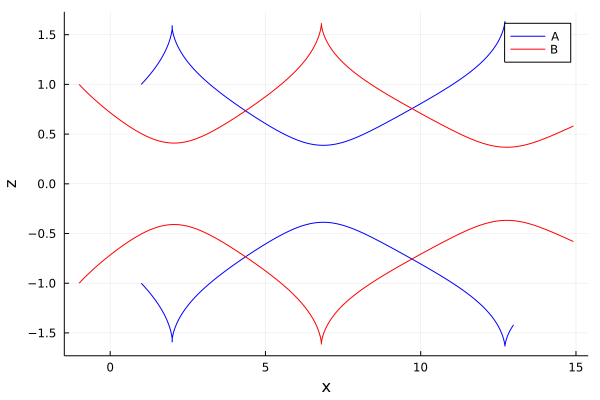
\includegraphics[width=\textwidth]{Graph_A.png}
	\caption{Paths of First Pair Leapfrogging Vortices\newline     This graph of the first set of vortices shows an ordinary case. These had the same vorticity, 1.0, and started out separated by exactly 2.0 in the x-direction. This graph shows that neglecting friction these vortices could continue in a straight line forever in the x-direction propelled only by leapfrogging.}
	\label{fig:vortexpaths}
\end{figure} 

\begin{figure}[htb]
	\centering
	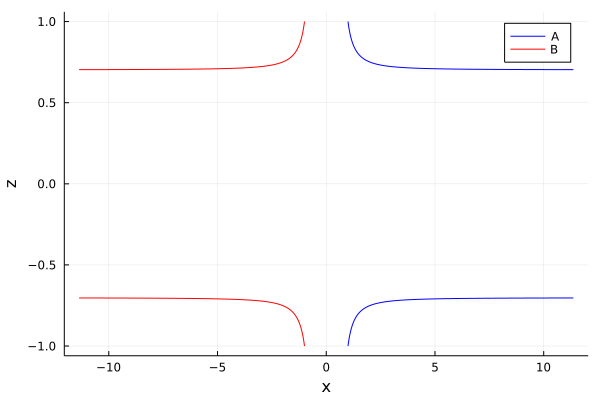
\includegraphics[width=\textwidth]{Graph_B.png}
	\caption{Second Pair of Leapfrogging Vortices\newline     This graph shows the second set of vortices. The only difference from the first pair is that these circulations are in opposite directions. instead of leapfrogging, the vortices get slightly smaller and are repelled by each other.}
	\label{fig:vortexpaths}
\end{figure} 

\begin{figure}[htb]
	\centering
	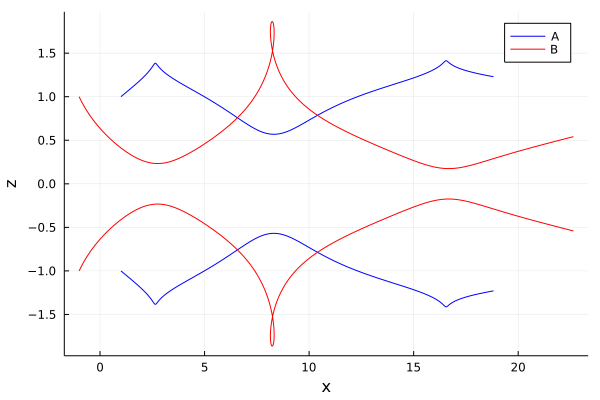
\includegraphics[width=\textwidth]{Graph_C.png}
	\caption{Third Pair of Leapfrogging Vortices\newline     In Figure 3, one vortex has a circulation twice as high as the other. This figure shows that they still leapfrog, but gradually grow further apart as one vortex pulls the other vortex further ahead while it stays behind.}
	\label{fig:vortexpaths}
\end{figure} 

\begin{figure}[htb]
	\centering
	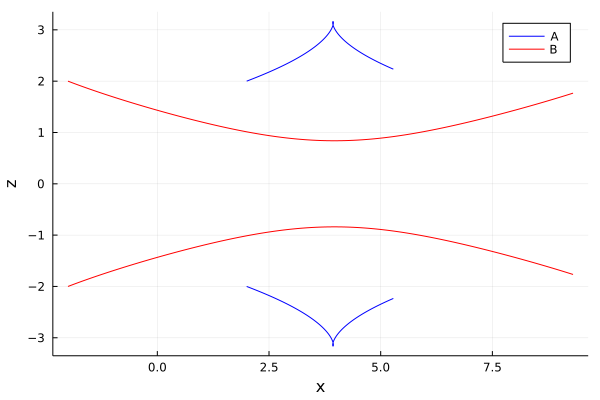
\includegraphics[width=\textwidth]{Graph_D.png}
	\caption{Fourth Pair of Leapfrogging Vortices\newline     The distance between the vortices was doubled in Figure 4. Comparison between Figure 4 and Figure 1 shows that in addition to the anticipated slower movement of the vortex pair, they did not change size as much through their paths as when they were twice as close to each other.}
	\label{fig:vortexpaths}
\end{figure} 

\begin{figure}[htb]
	\centering
	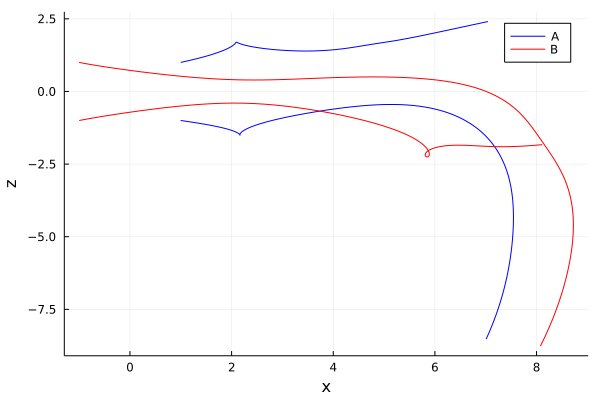
\includegraphics[width=\textwidth]{Graph_E.png}
	\caption{Fifth Pair of Leapfrogging Vortices\newline     One vortex in the fifth pair of leapfrogging vortices started out with an initial velocity in the x-direction and an initial velocity in the y-direction. The figure shows that it pulled the other vortex for a time, but eventually the leapfrogging vortex rings were broken. This shows that the vortices must be traveling at approximately the same velocity to exhibit leapfrogging.}
	\label{fig:vortexpaths}
\end{figure} 

\begin{figure}[htb]
	\centering
	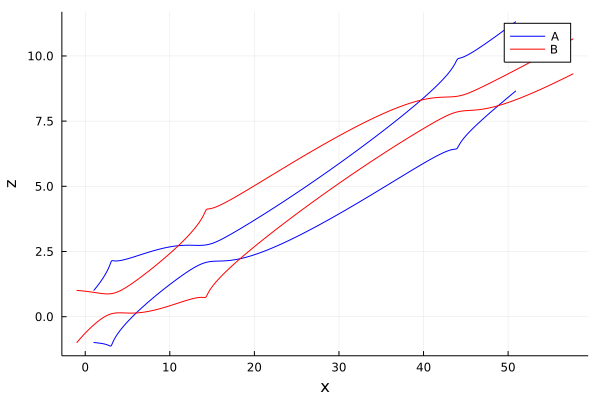
\includegraphics[width=\textwidth]{Graph_F.png}
	\caption{Sixth Pair of Leapfrogging Vortices\newline     Figure 6 takes Figure 5 a step further. The rings in Figure 6 travel in the same direction, but the direction they travel is not orthogonal to both the central axis of the vortices and their circulations. The vortices can be seen getting larger and larger and beginning to diverge paths towards the top right corner of the graphs. This proves that if the circulation and movement of vortices are not orthogonal to the line between them, they will eventually stop leapfrogging.}
	\label{fig:vortexpaths}
\end{figure} 

\begin{figure}[htb]
	\centering
	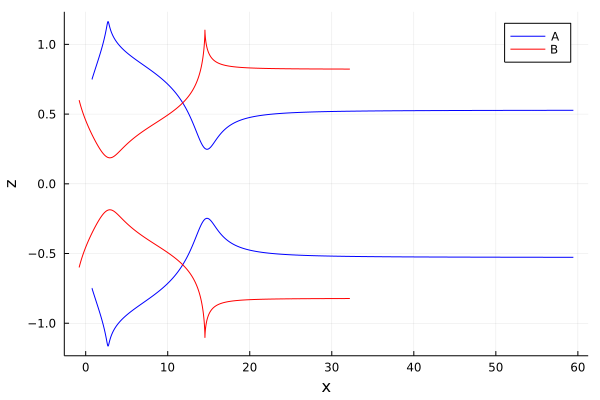
\includegraphics[width=\textwidth]{Graph_G.png}
	\caption{Seventh Pair of Leapfrogging Vortices\newline     In Figure 7, the blue vortex had an initial of 2, purely in the x-direction, while the red vortex had no starting velocity. This showed, similarly to Figure 5, that the initial velocities of a pair of vortices should be similar for it to leapfrog a longer time.}
	\label{fig:vortexpaths}
\end{figure} 

\end{document}